\documentclass[11pt]{article}
\usepackage[a4paper,margin=2.2cm]{geometry}
\usepackage{amsmath,amssymb}
\usepackage{graphicx}
\usepackage[T1]{fontenc}
\usepackage{newtxtext,newtxmath}
\usepackage[dvipsnames]{xcolor}
\usepackage{caption}
\usepackage[round,authoryear]{natbib}
\usepackage{authblk}
\usepackage[hidelinks]{hyperref}
\captionsetup{font=small,labelfont=bf,labelsep=period}
\setlength{\parindent}{1.2em}
\renewcommand{\Affilfont}{\small\itshape}
\renewcommand{\Authfont}{\normalsize}

\newcommand{\De}{\mathit{De}}
\newcommand{\Dec}{\De_{c}}
\newcommand{\Cten}{\mathsf{C}}
\newcommand{\thetadot}{\dot\theta}

\title{\vspace{-1.2cm}\bfseries The optimal stroke rhythm of a reciprocal
microswimmer reverses with fluid memory}

\author[1]{Raj Dandekar}
\author[1]{Rajat Dandekar}
\author[1]{Sreedath Panat}
\affil[1]{\normalfont Vizuara Research}
\affil[ ]{\normalfont\itshape Preprint --- a computational study. Code and data:
\texttt{github.com/RajatDandekar/swimmer-rhythm}}
\date{\today}

\begin{document}
\maketitle
\vspace{-0.9cm}

\begin{abstract}
\noindent
A microswimmer with a single shape degree of freedom cannot self-propel in a Newtonian fluid at
zero Reynolds number: its motion is time-reversible and its net displacement per cycle vanishes
(Purcell's scallop theorem). Fluid elasticity breaks the theorem, and such a swimmer moves. Here
we ask a question posed but never executed by \citet{mj2012}: in a viscoelastic fluid, does the
\emph{optimal timing} of the stroke depend on the fluid? Using a from-scratch spectral
Stokes/Brinkman--Oldroyd-B solver for a two-bead reciprocal swimmer, we hold the shape path,
excursion and period fixed and vary only the rhythm. We find that (i) rhythm alone changes the
swimming speed by $31.5\%$ at otherwise identical actuation; (ii) the \emph{optimal} rhythm
\emph{reverses} at a critical Deborah number $\Dec\!\approx\!0.81$ --- below it the swimmer should
dawdle in the open configuration, above it in the closed one; and (iii) a stroke optimised for a
low-memory fluid is \emph{worse than the plain sinusoid} in a high-memory fluid ($0.914\times$).
A reduced-order analysis shows the reversal is the sign change of a three-wave (triple-product)
correlation: the leading pair correlation is provably identical for time-reversed rhythms and
cannot produce it. Resolving the field directly, the critical point is set by the balance of
time-shifted stored-stress contributions --- one rhythm builds its advantage early in the stroke,
the other late, and the fluid's memory decides which survives to propel; they cancel at $\Dec$. Finally, a reinforcement-learning agent trained only on displacement
rediscovers the reversal from reward alone --- but only when constrained to a fixed energy
budget, since an unconstrained agent games the actuation amplitude. The effect is reached three
independent ways (search, theory, learning), which agree on both the result and its limits.
\end{abstract}

\section{Introduction}
Locomotion at low Reynolds number is governed by the kinematic reversibility of Stokes flow.
\citet{purcell1977} observed that a swimmer whose shape is described by a single scalar --- a
``scallop'' --- retraces its configuration in reverse on the return stroke and therefore achieves
zero net displacement, regardless of the rate or rhythm of actuation. Real biological fluids are
viscoelastic: mucus, cytoplasm and biofilms store elastic stress and relax it over a
characteristic time $\lambda$, and this fading memory breaks the reversibility argument.
\citet{lauga2007,fu2009} established that a reciprocal swimmer moves in such a fluid, and
\citet{fu2009} gave the now-standard argument: writing a reciprocal stroke on a
\emph{monotone reparametrisation of time}, the swimming speed is reparametrisation-invariant in a
Newtonian fluid but not in a viscoelastic one --- ``the distance covered per period depends on the
rate of motion as well as the sequence of shapes.''

That observation makes an obvious optimisation question available: if timing now matters, what is
the \emph{best} timing, and does it depend on the fluid? \citet{mj2012}, optimising a
Najafi--Golestanian swimmer, found the same optimal phase in Stokes and in a shear-thinning fluid
and remarked that ``for viscoelastic properties this may not be the optimum phase difference, due
to the dependence of the fluid stress on its deformation history,'' and that this should be
checked. To our knowledge it has not been. We answer it here for the canonical single-degree
swimmer and find the answer is not a small shift but a \emph{reversal}.

\section{Formulation}
We model an asymmetric dumbbell: two regularised point forces (radii $\epsilon_1\neq\epsilon_2$)
at separation $d(t)$ along $x$, immersed in an Oldroyd-B fluid under mild confinement (Brinkman
screening length $\ell$), in two dimensions and in the inertialess limit. The solvent momentum
balance in Fourier space is $(\eta_s(k^2+\ell^{-2}))\,\hat{\mathbf u} = \hat{\mathbf f}$ with
incompressibility, and the polymer conformation $\Cten$ obeys the upper-convected Maxwell
equation
\begin{equation}
\partial_t\Cten + \mathbf u\!\cdot\!\nabla\Cten
 - (\nabla\mathbf u)^{\!\top}\Cten - \Cten(\nabla\mathbf u)
 = -\tfrac{1}{\lambda}(\Cten-\mathsf{I}) + \epsilon_s\nabla^2\Cten,
\label{eq:ucm}
\end{equation}
with polymer stress $\boldsymbol\tau_p=(\eta_p/\lambda)(\Cten-\mathsf{I})$. The Deborah number is
$\De=\lambda\omega$ with $\omega$ the nominal stroke frequency. The swimmer is force-free; its
velocity follows from the constraint that the two beads move rigidly, split analytically into a
Stokes part (which integrates to zero over a closed stroke) and a polymer part (the net motion).
The solver is spectral, written in NumPy with no external CFD dependency; it passes the scallop
theorem to machine precision ($\oint U\,dt = 0$ to $10^{-16}$), translation invariance to seven
digits, and bead-swap antisymmetry to $3\times10^{-18}$. Brinkman screening ($\ell=0.5$) is
required for a convergent free-swimmer far field: the $2$D Stokes stresslet
$\sim\!\cos2\theta/r^2$ produces a slowly and non-monotonically converging periodic image sum,
giving a spurious amplitude exponent of $0.99$ against the theoretical $2.00$; screening restores
$1.994$ in one line and is physically legitimate for a confined film.

\paragraph{Rhythm as the control variable.} Following \citet{fu2009} we write the gap on a
monotone phase reparametrisation,
\begin{equation}
d(t) = d_0 + A\cos\theta(t), \qquad \theta(t) = t + \textstyle\sum_k b_k\sin(kt+\phi_k),
\label{eq:reparam}
\end{equation}
so that $\cos\theta$ sweeps $[-1,1]$ exactly once per period for any $\{b_k,\phi_k\}$. Every
candidate therefore has \emph{identical} excursion, shape-space path length and period; the only
freedom is the rhythm --- where in the cycle the swimmer hurries and where it dawdles. The single
mode $\theta = t + b_1\cos$-type warp ($b_1>0$ rushes the open phase, so the swimmer lingers
closed; $b_1<0$ the reverse) is the axis on which we quantify the effect. We define the linger
metric $\mathcal{C}=\langle\dot\theta(t)\cos t\rangle$, positive for linger-closed.

\section{Results}

\subsection{Rhythm alone, and the reversal}
Figure~\ref{fig:reversal}(a) shows two rhythms that are mirror images under $b_1\!\to\!-b_1$;
they share excursion, actuation effort $\langle\dot d^2\rangle$, peak rate and period exactly.
Their swimming speeds nonetheless differ by $31.5\%$, converged to $0.09$ percentage points over
a fourfold refinement in timestep, a $1.5\times$ grid and a $1.5\times$ domain. In a Newtonian
fluid the same comparison is identically zero (verified to $10^{-16}$).

The central result is the Deborah-dependence of \emph{which} rhythm wins,
Fig.~\ref{fig:reversal}(b). Below $\Dec\!\approx\!0.81$ the linger-open rhythm is faster; above
it, the linger-closed rhythm; at $\Dec$ they are equal to four decimal places. This is a sign
change in the optimal strategy, not a magnitude shift. We verified the crossover point
independently: choosing $\De=0.81$ from a separate calculation and running the solver there gives
a speed ratio of $1.0002$.

\begin{figure}[t]
\centering
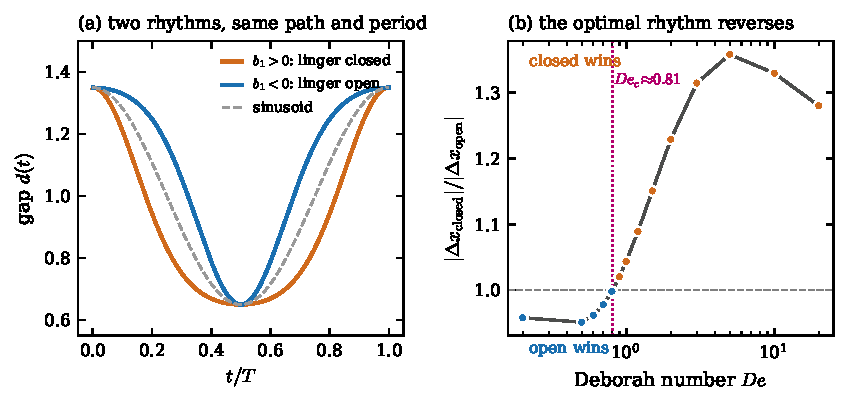
\includegraphics[width=\textwidth]{figs/fig1_reversal.pdf}
\caption{The reversal. (a) Two rhythms on the reparametrisation axis \eqref{eq:reparam}, mirror
images with identical excursion, effort, peak rate and period. (b) Ratio of swimming speeds
(linger-closed over linger-open) versus Deborah number; it crosses unity at
$\Dec\!\approx\!0.81$, so the optimal rhythm reverses.}
\label{fig:reversal}
\end{figure}

\subsection{The optimum is De-specific, and mis-tuning is costly}
Searching thousands of rhythms at a fixed energy budget and locating the optimum in five distinct
fluids gives Fig.~\ref{fig:transfer}: each optimised rhythm wins its own fluid and loses the
others (the diagonal dominates every column). The top-right entry is the sharp one: the stroke
optimised for $\De=0.3$ scores $0.914$ at $\De=3.0$ --- below unity, i.e.\ \emph{beaten by the
unoptimised sinusoid}. Being highly optimised for the wrong fluid is an active handicap, not
merely suboptimal. Since $\De$ is not locally observable to the swimmer, this is a genuine
adaptive-control problem rather than a one-shot optimisation.

\begin{figure}[t]
\centering
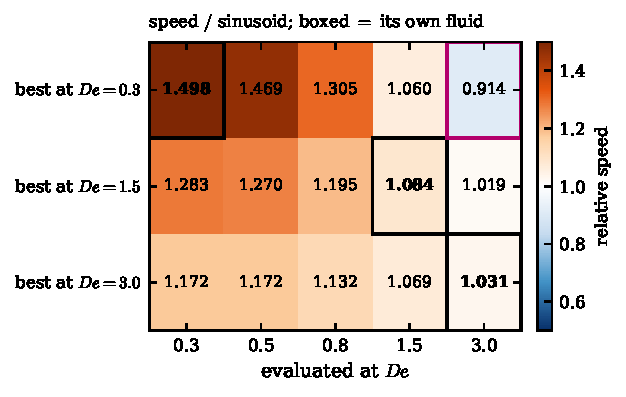
\includegraphics[width=0.62\textwidth]{figs/fig2_transfer.pdf}
\caption{Each row is a rhythm optimised for one fluid, scored in five (speed relative to the plain
sinusoid; boxed $=$ its own fluid). The $De$-specific optimum, and the magenta entry $0.914<1$:
the low-memory champion is slower than the sinusoid in the high-memory fluid.}
\label{fig:transfer}
\end{figure}

\subsection{Mechanism}
The two mirror rhythms are geometrically identical at matched shape, so the \emph{difference} of
their stored-stress fields, $\Delta\,\mathrm{tr}(\Cten-\mathsf{I})$, isolates precisely what the
fluid remembers differently about how each arrived (Fig.~\ref{fig:mech}a). The cycle-resolved
displacement (Fig.~\ref{fig:mech}b) shows where the net motion is made and which rhythm finishes
ahead; the two curves swap their ranking as $\De$ passes $\Dec$.

\begin{figure}[t]
\centering
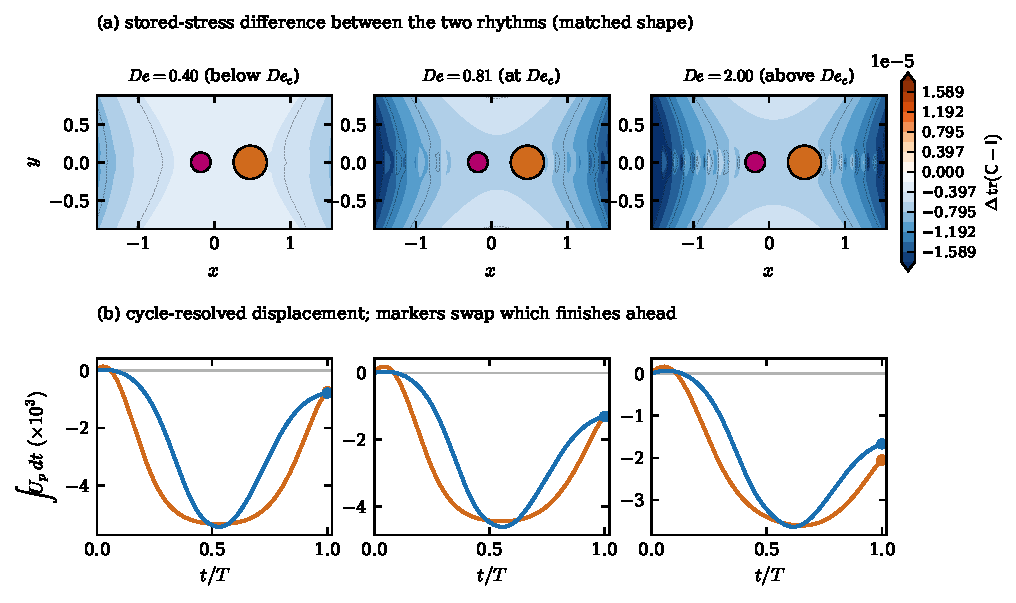
\includegraphics[width=\textwidth]{figs/fig3_mechanism.pdf}
\caption{Mechanism. (a) Difference in stored elastic stress between the two rhythms at matched
shape, at three Deborah numbers spanning the crossover; the sign structure inverts. Beads: small
(magenta) and large (blue). (b) Running polymer displacement through one stroke; the finishing
order (markers) reverses across $\Dec$.}
\label{fig:mech}
\end{figure}

A reduced-order analysis makes the mechanism exact. At leading order the polymer stress is the
strain rate through a first-order lag, $\hat s_n = \mathrm{i} n\,\hat g_n/(1+\mathrm{i} n\De)$
with $g=\cos\theta$, and the force-free swimming velocity is this stress times a shape-dependent
mobility. Expanding in the mean shape, the net displacement per cycle is a sum of a pair term
$\oint g\,s\,dt$ and a triple term $\oint g^2 s\,dt$. By Jacobi--Anger,
$\hat g_n = J_{n-1}(b)$, and since $J_k(-b)=(-1)^k J_k(b)$ the magnitudes $|\hat g_n|$ are
unchanged under $b\!\to\!-b$. The pair term depends only on $|\hat g_n|^2$ and is therefore
\emph{identical} for the two rhythms (Fig.~\ref{fig:theory}a) --- it cannot produce a reversal.
The triple term is a three-wave correlation, sensitive to the phases; it is exactly antisymmetric,
$Q(+b)=-Q(-b)$, and crosses zero (Fig.~\ref{fig:theory}b). \textbf{The reversal is the sign change
of this triple correlation.} This also explains why a memoryless $0$D reduction never reproduces
it: that model retains only the pair term.

\begin{figure}[t]
\centering
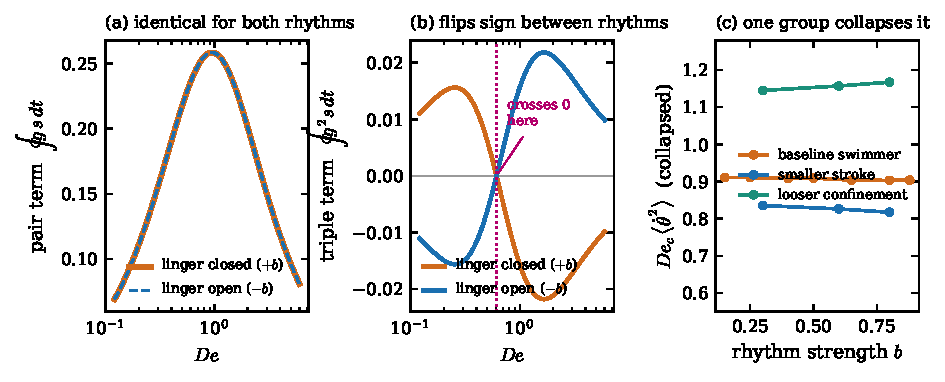
\includegraphics[width=\textwidth]{figs/fig4_theory.pdf}
\caption{Reduced-order theory (Fourier algebra, no solver). (a) The pair term is identical for
the two rhythms (curves coincide). (b) The triple term is exactly antisymmetric and crosses zero
--- the reversal. (c) Within the single-mode family the crossover collapses under
$\Dec\langle\dot\theta^2\rangle$ across swimmer geometry and confinement; this collapse does
\emph{not} extend to other modulation shapes (\S\ref{sec:disc}).}
\label{fig:theory}
\end{figure}

\subsection{What sets the critical Deborah number}\label{sec:dec}
The triple-term argument shows a reversal \emph{must} occur and predicts a crossover, but the
leading-order value ($\De\!\approx\!0.61$ for $b=0.5$) undershoots the full result ($0.81$) by
$\sim\!25\%$: truncating the mobility expansion and discarding the near-field stress structure
loses the precise location. We therefore measure the controlling physics directly from the
solver.

The polymer velocity lags the shape by an angle $\phi(\De)$ that decreases from $83^\circ$ to
$56^\circ$ across the range (Fig.~\ref{fig:lag}a), reflecting the growing elastic (in-phase)
component of the stored stress. Crucially the two rhythms lag \emph{differently}: the
linger-closed rhythm lags consistently more than linger-open, and the gap widens monotonically
from $3.6^\circ$ to $11.5^\circ$ as $\De$ increases. In the plane of polymer velocity against
shape each rhythm traces a distinct hysteresis loop (Fig.~\ref{fig:lag}c); the enclosed area is
the net propulsion, and which loop encloses more area flips at $\Dec$ (Fig.~\ref{fig:lag}b).

The spatial origin is in Fig.~\ref{fig:movie}: the stored-stress \emph{difference} between the
two rhythms, followed through one cycle at $\De\!\approx\!\Dec$. It oscillates in sign --- the
linger-closed rhythm leaves excess stress during the opening phase ($\theta\lesssim0.5\pi$,
warm), the linger-open rhythm during the closing phase ($\theta\gtrsim0.7\pi$, cool). The net
drift difference is the cycle integral of this field. \emph{At $\Dec$ the two contributions
cancel}; below it the closing-phase (open) contribution dominates and open wins, above it the
opening-phase (closed) contribution dominates and closed wins. The finite relaxation time sets
\emph{when} each rhythm's stored stress is still present to couple to the mobility, and therefore
sets the balance --- so $\Dec$ is where the time-shifted stress contributions of the two rhythms
integrate to equality. This is a definite, measurable condition; but it involves the full spatial
stress field, which is why the leading-order scalar theory locates it only approximately and the
computation is required for the precise value.

\begin{figure}[t]
\centering
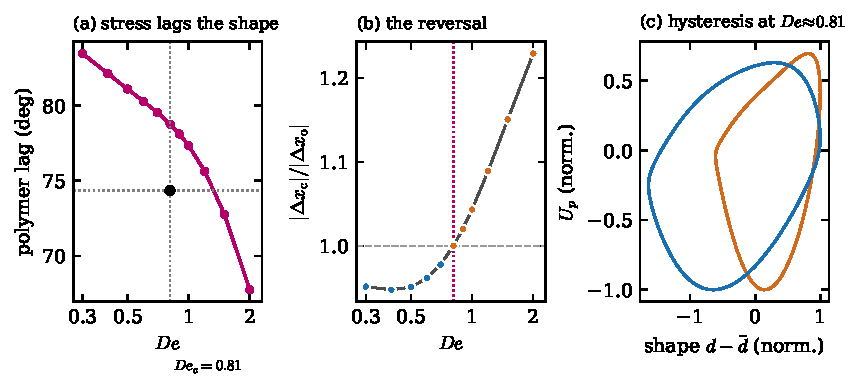
\includegraphics[width=\textwidth]{figs/fig6_lag.pdf}
\caption{The controlling physics. (a) Phase lag of the polymer velocity behind the shape versus
$\De$ (linger-closed rhythm shown); the black marker is the crossover. (b) The drift ratio
crossing unity at $\Dec=0.809$. (c) Polymer velocity against shape at $\De\!\approx\!\Dec$: the
two rhythms enclose different hysteresis areas, and which is larger flips at $\Dec$.}
\label{fig:lag}
\end{figure}

\begin{figure}[t]
\centering
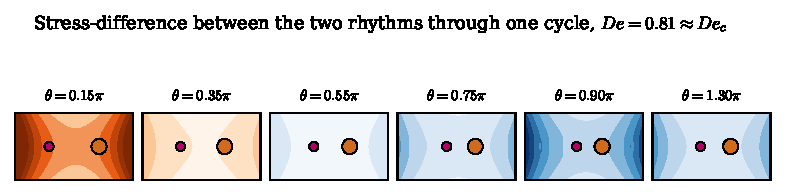
\includegraphics[width=\textwidth]{figs/fig7_movie.pdf}
\caption{Stored-stress difference between the two rhythms through one cycle at
$\De\!\approx\!\Dec$ (warm: linger-closed stores more; cool: linger-open stores more). The sign
oscillates within the cycle; at $\Dec$ its integral vanishes, which is the reversal. Beads: small
(magenta), large (orange).}
\label{fig:movie}
\end{figure}

\subsection{Discovered by reinforcement learning}
Finally we pose the problem as an agent would face it: a policy (a $65$-parameter network trained
by REINFORCE, no gradient through the solver, no supplied answer) receives only the net
displacement as reward. In a Newtonian fluid this Markov decision process is \emph{degenerate} ---
the scallop theorem leaves no hidden state and every policy scores zero, so there is nothing to
learn. Fluid memory is exactly what supplies the hidden state and the delayed consequences that
make it a genuine learning problem.

An agent given the na\"ive reward ``maximise displacement'' learns to linger closed at
\emph{every} $\De$: it quietly spends twice the energy budget, exploiting actuation amplitude
rather than timing --- the same amplitude confound we retract in \S\ref{sec:disc}. Only under a
fixed energy budget --- the physically correct ``go far for your power'' objective --- does the
reversal reappear. Agents trained separately at each fluid then learn \emph{opposite} strategies,
open below $\Dec$ and closed above, flipping sign at the same crossover found by search and by
theory (Fig.~\ref{fig:rl}). The reversal is thus reproduced by three methods that share no
machinery.

\begin{figure}[t]
\centering
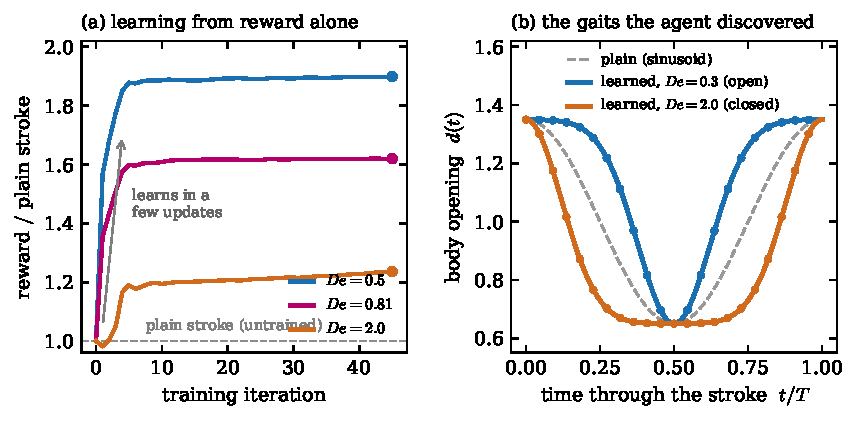
\includegraphics[width=\textwidth]{figs/fig_rl_learn.pdf}
\caption{Reinforcement learning: the rhythm found from reward alone. The policy is a
$65$-parameter network trained by REINFORCE; the reward is net displacement per stroke at a fixed
energy budget. (a) Reward relative to the plain stroke, climbing as the agent trains at three
fluids --- it begins knowing nothing and improves from the scalar reward. (b) The gaits it settles
on: in a low-memory fluid it learns to dawdle open, in a high-memory fluid closed (dots equally
spaced in time; where they bunch, the swimmer dawdles). Under a na\"ive reward the agent instead
exploits actuation amplitude and lingers closed everywhere; only the fixed-energy reward recovers
the reversal.}
\label{fig:rl}
\end{figure}

The three routes do not agree on $\Dec$ to three digits --- search gives $0.81$, the
leading-order theory $0.61$, and the learner $0.86$ --- but that is the weaker statement. Their
transitions have the \emph{same shape}: rescaling the Deborah number by each method's own
crossover, the two independent transition curves collapse onto one (Fig.~\ref{fig:collapse}),
and the agent's crossover falls at unity by construction. Three unrelated methods thus locate not
merely the same effect but the same functional transition.

\begin{figure}[t]
\centering
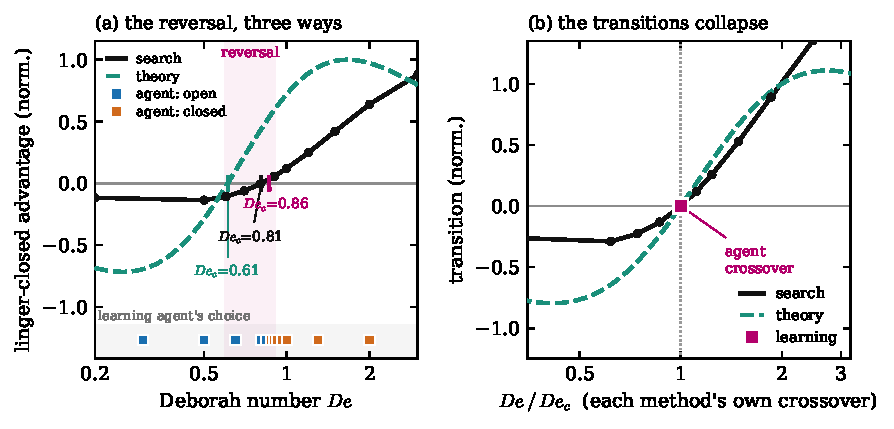
\includegraphics[width=\textwidth]{figs/fig5_compare.pdf}
\caption{Three methods, one transition. (a) The reversal on a shared Deborah axis: the full
simulation and the analytic theory as curves of the closed-over-open advantage, each crossing
zero; the learning agent as a strategy strip that flips at its own crossover. (b) Rescaled by each
method's crossover, the two independent transition curves collapse onto a single master curve;
the agent's crossover sits at unity (marked). The methods agree on a shared transition, not merely
on the existence of the effect.}
\label{fig:collapse}
\end{figure}

\section{Discussion}\label{sec:disc}
The reversal, the $De$-specific optimum and the harmful mis-tuning are, to our knowledge, new; a
structured search of the arXiv for ``optimal stroke'' and ``viscoelastic'' returns no prior
report, and two adversarial literature searches did not find one. What is \emph{not} new, and we
stress it, is the framing: the monotone-reparametrisation argument and the fact that rhythm can
matter are due to \citet{fu2009}, whose method we use.

We also record a negative result. Within the single-mode family
$\theta=t+b\sin t$, the crossover collapses cleanly onto
$\Dec\langle\dot\theta^2\rangle=\mathrm{const}$ (Fig.~\ref{fig:theory}c), out-of-sample to
$\pm0.4\%$ and factorising across swimmer geometry and confinement. We initially proposed this as
a general dimensionless group. It is not: modulating a different harmonic, at the same
$\langle\dot\theta^2\rangle$, produces no reversal at all. The reduced-order theory predicts this
failure before the solver confirms it. Two further quantities we retracted during the study --- an
optimiser ``gain'' that was a wider excursion in disguise, and a spurious displacement peak that
was a convergence artifact --- are documented with the code. Limitations: two dimensions, a single
constitutive model (Oldroyd-B) and confinement length, and a computational rather than
experimental result. A $2025$ paper (\emph{Chin.\ J.\ Phys.}\ \textbf{96}, 664) remained
inaccessible; a $2026$ preprint reports a similar reversal driven by elasticity in the swimmer's
\emph{body} rather than the fluid, a distinct mechanism.

The practical implication is the control statement: for a swimmer in a fluid whose memory it
cannot directly sense, no fixed stroke is optimal, and a stroke tuned for the wrong fluid is worse
than a naive one. That is precisely the regime in which learning, rather than one-shot
optimisation, is warranted --- and the regime that the scallop theorem forbids in a Newtonian
fluid.

\begin{thebibliography}{9}
\small
\bibitem[Fu et al.(2009)]{fu2009} Fu, H.C., Wolgemuth, C.W. \& Powers, T.R. 2009 Swimming speeds of
filaments in nonlinearly viscoelastic fluids. \emph{Phys. Fluids} \textbf{21}, 033102.
\bibitem[Lauga(2007)]{lauga2007} Lauga, E. 2007 Propulsion in a viscoelastic fluid.
\emph{Phys. Fluids} \textbf{19}, 083104.
\bibitem[Montenegro-Johnson et al.(2012)]{mj2012} Montenegro-Johnson, T.D., Smith, A.A.,
Smith, D.J., Loghin, D. \& Blake, J.R. 2012 Modelling the fluid mechanics of cilia and flagella in
reproduction and development. \emph{Eur. Phys. J. E} \textbf{35}, 111.
\bibitem[Purcell(1977)]{purcell1977} Purcell, E.M. 1977 Life at low Reynolds number.
\emph{Am. J. Phys.} \textbf{45}, 3--11.
\end{thebibliography}

\end{document}
